\documentclass[11pt,a4paper]{article}
% Build:  python documentation/make_report_assets.py  &&  (cd documentation && tectonic fairfare_report.tex)
%         (pdflatex works too: run it twice)
\usepackage[T1]{fontenc}
\usepackage[utf8]{inputenc}
\usepackage{lmodern}
\usepackage[margin=2.4cm]{geometry}
\usepackage{amsmath,amssymb}
\usepackage{booktabs}
\usepackage{graphicx}
\usepackage{caption}
\usepackage{subcaption}
\usepackage{xcolor}
\usepackage{microtype}
\usepackage{enumitem}
\usepackage{array}
\usepackage[hidelinks]{hyperref}
\captionsetup{font=small,labelfont=bf}
\setlist{nosep,leftmargin=1.4em}
\definecolor{olive}{HTML}{7D6400}
\graphicspath{{figures/}}
% generated by make_report_assets.py -- do not edit
\newcommand{\JulyN}{128,359}
\newcommand{\JulyFinalMae}{\POSNUM{2.002}}
\newcommand{\JulyFinalRmse}{\POSNUM{2.959}}
\newcommand{\JulyFinalBias}{\NEGNUM{0.105}}
\newcommand{\JulyMedianMae}{\POSNUM{7.716}}
\newcommand{\JulyMedianRmse}{\POSNUM{12.239}}
\newcommand{\JulyMedianBias}{\POSNUM{3.137}}
\newcommand{\JulyRuleMae}{\POSNUM{2.828}}
\newcommand{\JulyRuleRmse}{\POSNUM{3.796}}
\newcommand{\JulyRuleBias}{\NEGNUM{0.479}}
\newcommand{\JulyTlcMae}{\POSNUM{4.496}}
\newcommand{\JulyTlcRmse}{\POSNUM{5.949}}
\newcommand{\JulyTlcBias}{\POSNUM{4.484}}
\newcommand{\JulyVsMedianMaemodelPoint}{\POSNUM{2.002}}
\newcommand{\JulyVsMedianMaemodelLo}{\POSNUM{1.925}}
\newcommand{\JulyVsMedianMaemodelHi}{\POSNUM{2.086}}
\newcommand{\JulyVsMedianMaediffPoint}{\NEGNUM{5.714}}
\newcommand{\JulyVsMedianMaediffLo}{\NEGNUM{5.851}}
\newcommand{\JulyVsMedianMaediffHi}{\NEGNUM{5.574}}
\newcommand{\JulyVsMedianRmsemodelPoint}{\POSNUM{2.959}}
\newcommand{\JulyVsMedianRmsemodelLo}{\POSNUM{2.823}}
\newcommand{\JulyVsMedianRmsemodelHi}{\POSNUM{3.124}}
\newcommand{\JulyVsMedianRmsediffPoint}{\NEGNUM{9.280}}
\newcommand{\JulyVsMedianRmsediffLo}{\NEGNUM{9.509}}
\newcommand{\JulyVsMedianRmsediffHi}{\NEGNUM{9.048}}
\newcommand{\JulyVsMedianMaebaselinePoint}{\POSNUM{7.716}}
\newcommand{\JulyVsMedianMaebaselineLo}{\POSNUM{7.591}}
\newcommand{\JulyVsMedianMaebaselineHi}{\POSNUM{7.837}}
\newcommand{\JulyVsRuleMaemodelPoint}{\POSNUM{2.002}}
\newcommand{\JulyVsRuleMaemodelLo}{\POSNUM{1.925}}
\newcommand{\JulyVsRuleMaemodelHi}{\POSNUM{2.086}}
\newcommand{\JulyVsRuleMaediffPoint}{\NEGNUM{0.826}}
\newcommand{\JulyVsRuleMaediffLo}{\NEGNUM{0.876}}
\newcommand{\JulyVsRuleMaediffHi}{\NEGNUM{0.770}}
\newcommand{\JulyVsRuleRmsemodelPoint}{\POSNUM{2.959}}
\newcommand{\JulyVsRuleRmsemodelLo}{\POSNUM{2.823}}
\newcommand{\JulyVsRuleRmsemodelHi}{\POSNUM{3.124}}
\newcommand{\JulyVsRuleRmsediffPoint}{\NEGNUM{0.837}}
\newcommand{\JulyVsRuleRmsediffLo}{\NEGNUM{0.897}}
\newcommand{\JulyVsRuleRmsediffHi}{\NEGNUM{0.769}}
\newcommand{\JulyVsRuleMaebaselinePoint}{\POSNUM{2.828}}
\newcommand{\JulyVsRuleMaebaselineLo}{\POSNUM{2.758}}
\newcommand{\JulyVsRuleMaebaselineHi}{\POSNUM{2.906}}
\newcommand{\JulyQuoteCoverage}{\POSNUM{0.926}}
\newcommand{\JulyQuoteMeanoverquote}{\POSNUM{4.250}}
\newcommand{\JulyQuoteMeancushion}{\POSNUM{4.032}}
\newcommand{\JulyQuoteMeanshortfallwhenunder}{\POSNUM{2.937}}
\newcommand{\JulyScoredAt}{2026-11-15 18:36:37}
\newcommand{\JuneFinalMae}{\POSNUM{2.082}}
\newcommand{\JuneFinalRmse}{\POSNUM{3.234}}
\newcommand{\JuneFinalBias}{\POSNUM{0.421}}
\newcommand{\JuneMedianMae}{\POSNUM{7.901}}
\newcommand{\JuneMedianRmse}{\POSNUM{12.552}}
\newcommand{\JuneMedianBias}{\POSNUM{3.419}}
\newcommand{\JuneRuleMae}{\POSNUM{2.979}}
\newcommand{\JuneRuleRmse}{\POSNUM{4.151}}
\newcommand{\JuneRuleBias}{\NEGNUM{0.061}}
\newcommand{\JuneTlcMae}{\POSNUM{4.894}}
\newcommand{\JuneTlcRmse}{\POSNUM{6.552}}
\newcommand{\JuneTlcBias}{\POSNUM{4.885}}
\newcommand{\JuneSkeletonMae}{\POSNUM{2.590}}
\newcommand{\JuneSkeletonRmse}{\POSNUM{3.672}}
\newcommand{\JuneSkeletonBias}{\NEGNUM{0.070}}
\newcommand{\JuneTreetwoMae}{\POSNUM{3.948}}
\newcommand{\JuneTreetwoRmse}{\POSNUM{5.425}}
\newcommand{\JuneTreetwoBias}{\NEGNUM{0.079}}
\newcommand{\JuneQuoteCoverage}{\POSNUM{0.900}}
\newcommand{\JuneQuoteMeanoverquote}{\POSNUM{3.829}}
\newcommand{\JuneQuoteMeancushion}{\POSNUM{3.495}}
\newcommand{\JuneQuoteMeanshortfallwhenunder}{\POSNUM{3.331}}
\newcommand{\ParamLoss}{absolute\_error}
\newcommand{\ParamLearningrate}{0.1}
\newcommand{\ParamMaxleafnodes}{127}
\newcommand{\ParamMaxiter}{300}
\newcommand{\ParamMinsamplesleaf}{100}
\newcommand{\SelTreeMaePoint}{\NEGNUM{0.290}}
\newcommand{\SelTreeMaeLo}{\NEGNUM{0.312}}
\newcommand{\SelTreeMaeHi}{\NEGNUM{0.269}}
\newcommand{\SelLinearMaePoint}{\NEGNUM{0.374}}
\newcommand{\SelLinearMaeLo}{\NEGNUM{0.399}}
\newcommand{\SelLinearMaeHi}{\NEGNUM{0.346}}
\newcommand{\SelRuleMaePoint}{\NEGNUM{0.897}}
\newcommand{\SelRuleMaeLo}{\NEGNUM{0.946}}
\newcommand{\SelRuleMaeHi}{\NEGNUM{0.842}}
\newcommand{\RouterK}{\POSNUM{1.238}}
\newcommand{\RouterDistMae}{\POSNUM{0.532}}
\newcommand{\RouterDistMape}{\POSNUM{19.0}}
\newcommand{\RouterOdoMae}{\POSNUM{2.082}}
\newcommand{\RouterOdoCov}{\POSNUM{90.0}}
\newcommand{\RouterEstMae}{\POSNUM{3.255}}
\newcommand{\RouterEstCov}{\POSNUM{82.2}}
\newcommand{\RouterRetrainedMae}{\POSNUM{2.939}}
\newcommand{\RouterRetrainedCov}{\POSNUM{85.2}}
\newcommand{\RouterPairMae}{\POSNUM{3.037}}
\newcommand{\RouterPairCov}{\POSNUM{83.3}}
\newcommand{\RouterXfitCov}{\POSNUM{90.0}}
\newcommand{\RouterXfitCushion}{\POSNUM{5.27}}
\newcommand{\MayFareMean}{\POSNUM{16.88}}
\newcommand{\MayFareMedian}{\POSNUM{13.50}}
\newcommand{\MayFareQone}{\POSNUM{9.30}}
\newcommand{\MayFareQthree}{\POSNUM{20.50}}
\newcommand{\MayFareStd}{\POSNUM{11.92}}
\newcommand{\MayN}{133,342}
\newcommand{\SlowShare}{\POSNUM{22.9}}
\newcommand{\SlowFpm}{\POSNUM{12.23}}
\newcommand{\MedianFpm}{\POSNUM{7.90}}

% generated by make_report_assets.py -- do not edit
\newcommand{\TableCleaning}{%
\begin{table}[htbp]\centering\small
\caption{Population definition. Removals are sequential; percentages are of each month's raw trips. Caps fitted on May (distance 24.85 mi, fare \$96.80) and reused for June and July.}\label{tab:cleaning}
\begin{tabular}{lrrrr}\toprule
Rule (applied in order) & Removed (May) & \% May & \% June & \% July \\ \midrule
Unknown/missing zone (264, 265) & 1,271 & 0.64 & 0.72 & 0.77 \\
Flex fare (payment type 0) & 46,429 & 23.21 & 26.31 & 27.38 \\
Payment not card or cash & 1,650 & 0.82 & 0.85 & 0.86 \\
Rate code $\neq$ 1 & 13,493 & 6.75 & 3.46 & 5.02 \\
Fare $\leq$ 0 & 195 & 0.10 & 0.11 & 0.12 \\
Distance $\leq$ 0 & 725 & 0.36 & 0.39 & 0.38 \\
Duration $<1$ or $>180$ min & 2,729 & 1.36 & 1.35 & 1.20 \\
Above May 99.9\% caps & 165 & 0.08 & 0.08 & 0.09 \\
\bottomrule\end{tabular}
\par\smallskip\begin{minipage}{0.92\linewidth}\footnotesize Kept: May 133,342, June 133,459, July 128,359 trips; 2 pickups outside May--July dropped before the split.\end{minipage}
\end{table}
}
\newcommand{\TableSummary}{%
\begin{table}[htbp]\centering\small
\caption{Descriptive statistics of the cleaned May (training) trips, $n=133,342$.}\label{tab:summary}
\begin{tabular}{lrrrrrrr}\toprule
Measure & Mean & SD & Min & Q1 & Median & Q3 & Max \\ \midrule
Fare (\$) & 16.88 & 11.92 & 3.00 & 9.30 & 13.50 & 20.50 & 96.80 \\
Distance (mi) & 2.56 & 2.80 & 0.01 & 0.98 & 1.60 & 2.80 & 24.85 \\
Duration (min)$^\dagger$ & 15.59 & 11.06 & 1.00 & 7.87 & 12.73 & 20.17 & 159.77 \\
Fare per mile (\$)$^\dagger$ & 8.87 & 6.81 & 0.75 & 6.26 & 7.90 & 10.09 & 510.00 \\
Speed (mph)$^\dagger$ & 9.49 & 5.29 & 0.01 & 6.20 & 8.36 & 11.25 & 82.62 \\
\bottomrule\end{tabular}
\par\smallskip\begin{minipage}{0.92\linewidth}\footnotesize $^\dagger$ Measured after the trip; used to describe fares, never as model inputs.\end{minipage}
\end{table}
}
\newcommand{\TableQuartiles}{%
\begin{table}[htbp]\centering\small
\caption{Fare quartiles (\$) by trip type, May.}\label{tab:quartiles}
\begin{tabular}{llrrrrrr}\toprule
Group & Level & $n$ & Mean & Q1 & Median & Q3 & Median \$/mi \\ \midrule
Distance & 0-1 mi & 35,797 & 8.05 & 6.50 & 7.20 & 9.30 & 10.85 \\
 & 1-2 mi & 46,607 & 12.58 & 10.00 & 12.10 & 14.20 & 8.16 \\
 & 2-5 mi & 34,931 & 20.16 & 16.30 & 19.10 & 23.30 & 6.53 \\
 & 5-10 mi & 11,348 & 35.99 & 30.30 & 35.20 & 40.80 & 4.82 \\
 & 10-20 mi & 4,503 & 55.56 & 47.10 & 53.40 & 62.50 & 4.26 \\
 & 20+ mi & 156 & 84.68 & 80.70 & 84.20 & 88.40 & 3.87 \\
Time of day & night 0-5 & 9,540 & 16.61 & 8.60 & 12.80 & 20.50 & 6.22 \\
 & am 6-9 & 14,762 & 15.74 & 8.60 & 12.10 & 17.70 & 7.50 \\
 & midday 10-15 & 44,427 & 17.50 & 9.30 & 13.50 & 21.20 & 8.73 \\
 & pm 16-19 & 36,413 & 16.58 & 9.30 & 13.50 & 19.80 & 8.33 \\
 & eve 20-23 & 28,200 & 16.98 & 9.30 & 13.50 & 20.50 & 7.05 \\
Day & weekday & 93,715 & 17.10 & 9.30 & 13.50 & 20.50 & 8.12 \\
 & weekend & 39,627 & 16.37 & 8.60 & 12.80 & 19.80 & 7.43 \\
Airport & airport trip & 8,856 & 45.31 & 36.60 & 44.30 & 54.10 & 4.38 \\
 & non-airport & 124,486 & 14.86 & 8.60 & 12.80 & 18.40 & 8.12 \\
\bottomrule\end{tabular}
\end{table}
}
\newcommand{\TableRankzone}{%
\begin{table}[htbp]\centering\footnotesize
\caption{The five highest and five lowest May pickup zones ranked by median fare ($n\geq200$).}\label{tab:rank-zone}
\resizebox{\linewidth}{!}{%
\begin{tabular}{lp{0.5\linewidth}rrrrrr}\toprule
 & Pickup zone & $n$ & Med.\ fare & Med.\ mi & Med.\ min & Med.\ mph & \$/mi \\ \midrule
top & LaGuardia Airport (Queens) & 4,656 & 44.30 & 9.3 & 34 & 16.4 & 4.56 \\
top & JFK Airport (Queens) & 2,863 & 42.90 & 10.4 & 27 & 22.8 & 4.17 \\
top & East Elmhurst (Queens) & 350 & 42.20 & 9.0 & 32 & 17.4 & 4.46 \\
top & Financial District South (Manhattan) & 410 & 21.20 & 3.8 & 17 & 11.3 & 5.86 \\
top & World Trade Center (Manhattan) & 560 & 19.80 & 3.0 & 18 & 10.2 & 6.52 \\
bottom & Lenox Hill West (Manhattan) & 3,431 & 10.70 & 1.3 & 10 & 8.3 & 8.23 \\
bottom & Yorkville West (Manhattan) & 2,639 & 10.70 & 1.4 & 9 & 9.3 & 7.65 \\
bottom & Upper East Side North (Manhattan) & 7,091 & 10.70 & 1.3 & 10 & 8.0 & 8.42 \\
bottom & Upper East Side South (Manhattan) & 8,556 & 10.70 & 1.2 & 10 & 7.5 & 8.86 \\
bottom & Lincoln Square West (Manhattan) & 1,474 & 11.40 & 1.6 & 11 & 8.9 & 7.75 \\
\bottomrule\end{tabular}}
\end{table}
}
\newcommand{\TableRankfpm}{%
\begin{table}[htbp]\centering\footnotesize
\caption{The five highest and five lowest May routes ranked by median fare per mile ($n\geq50$).}\label{tab:rank-fpm}
\resizebox{\linewidth}{!}{%
\begin{tabular}{lp{0.5\linewidth}rrrrrr}\toprule
 & Route & $n$ & Med.\ fare & Med.\ mi & Med.\ min & Med.\ mph & \$/mi \\ \midrule
top & Times Sq/Theatre District (Manhattan) $\rightarrow$ Times Sq/Theatre District (Manhattan) & 134 & 8.25 & 0.5 & 8 & 4.0 & 15.74 \\
top & Midtown South (Manhattan) $\rightarrow$ Midtown South (Manhattan) & 63 & 6.50 & 0.4 & 6 & 4.9 & 15.49 \\
top & Midtown Center (Manhattan) $\rightarrow$ Times Sq/Theatre District (Manhattan) & 202 & 10.00 & 0.7 & 10 & 3.9 & 15.38 \\
top & Midtown Center (Manhattan) $\rightarrow$ Midtown Center (Manhattan) & 268 & 7.20 & 0.5 & 6 & 4.6 & 14.93 \\
top & Midtown East (Manhattan) $\rightarrow$ Midtown Center (Manhattan) & 159 & 8.60 & 0.6 & 8 & 4.1 & 14.79 \\
bottom & JFK Airport (Queens) $\rightarrow$ Flushing Meadows-Corona Park (Queens) & 176 & 31.70 & 8.2 & 14 & 34.5 & 3.90 \\
bottom & JFK Airport (Queens) $\rightarrow$ LaGuardia Airport (Queens) & 68 & 44.30 & 11.5 & 27 & 24.3 & 4.02 \\
bottom & JFK Airport (Queens) $\rightarrow$ Williamsburg (North Side) (Brooklyn) & 69 & 66.00 & 15.8 & 46 & 21.0 & 4.08 \\
bottom & JFK Airport (Queens) $\rightarrow$ Greenpoint (Brooklyn) & 54 & 64.60 & 15.5 & 46 & 21.1 & 4.09 \\
bottom & JFK Airport (Queens) $\rightarrow$ Briarwood/Jamaica Hills (Queens) & 53 & 23.30 & 5.7 & 13 & 27.2 & 4.09 \\
\bottomrule\end{tabular}}
\end{table}
}
\newcommand{\TableAblation}{%
\begin{table}[htbp]\centering\small
\caption{Feature ablation: June MAE (\$) of models trained on May with default hyperparameters. Sets are cumulative.}\label{tab:ablation}
\begin{tabular}{llrrr}\toprule
Set & Adds & OLS & Tree & HGB \\ \midrule
\texttt{f0\_distance} & distance & 2.979 & 2.793 & 2.800 \\
\texttt{f1\_time} & + hour, weekday & 2.819 & 2.770 & 2.499 \\
\texttt{f2\_geo} & + boroughs, same zone/borough & 2.733 & 2.747 & 2.444 \\
\texttt{f3\_airport} & + airport flags & 2.719 & 2.747 & 2.441 \\
\texttt{f4\_shape} & + log distance, distance band & 2.590 & 2.747 & 2.434 \\
\texttt{f5\_zones} & + PU/DO zone (target enc.) & 2.577 & 2.699 & 2.259 \\
\texttt{f6\_pair} & + zone pair (target enc.) & 2.525 & 2.633 & 2.190 \\
\texttt{f7\_time\_x} & + hour$\times$weekend, distance$\times$time band & 2.455 & 2.536 & 2.169 \\
\bottomrule\end{tabular}
\end{table}
}
\newcommand{\TableSelection}{%
\begin{table}[htbp]\centering\small
\caption{Candidates at their best feature set and June-tuned hyperparameters.}\label{tab:selection}
\begin{tabular}{lrrr}\toprule
Candidate (tuned, June) & MAE & RMSE & Bias \\ \midrule
rate rule (TLC \$3 + \$3.50/mi) & 4.894 & 6.552 & +4.885 \\
rate rule (fit on May) & 2.979 & 4.151 & -0.061 \\
linear f7 & 2.455 & 3.540 & -0.081 \\
tree f7 (depth 20, leaf 50) & 2.372 & 3.482 & -0.102 \\
hgb f7 (chosen params) & 2.082 & 3.234 & +0.421 \\
\bottomrule\end{tabular}
\end{table}
}
\newcommand{\TableLadder}{%
\begin{table}[htbp]\centering\small
\caption{Baseline ladder and final model. June: validation; July: test, scored once ($n=128,359$). Bias $=\overline{y-\hat y}$.}\label{tab:ladder}
\resizebox{\linewidth}{!}{%
\begin{tabular}{lrrrrr}\toprule
Model & June MAE & June bias & July MAE & July RMSE & July bias \\ \midrule
May median fare & 7.901 & +3.419 & 7.716 & 12.239 & +3.137 \\
TLC rule, distance only (\$3 + \$3.50/mi) & 4.894 & +4.885 & 4.496 & 5.949 & +4.484 \\
Rate rule fitted on May & 2.979 & -0.061 & 2.828 & 3.796 & -0.479 \\
Depth-2 tree & 3.948 & -0.079 & 3.816 & 5.173 & -0.480 \\
OLS, \texttt{f4\_shape} & 2.590 & -0.070 & 2.512 & 3.390 & -0.560 \\
\textbf{Fairfare (HGB, \texttt{f7\_time\_x})} & 2.082 & +0.421 & 2.002 & 2.959 & -0.105 \\
\bottomrule\end{tabular}}
\end{table}
}
\newcommand{\TableSlices}{%
\begin{table}[htbp]\centering\footnotesize
\caption{July slices of the final model with the frozen quote rule (slices with $n<50$ omitted).}\label{tab:slices}
\begin{tabular}{llrrrr}\toprule
Slice & Level & $n$ & MAE & Bias & Coverage \\ \midrule
Distance (mi) & 0-1 & 34,506 & 1.39 & +0.19 & 91.3\% \\
 & 1-2 & 43,944 & 1.84 & -0.12 & 92.7\% \\
 & 2-5 & 33,685 & 2.38 & -0.30 & 93.4\% \\
 & 5-10 & 11,228 & 2.74 & -0.34 & 93.7\% \\
 & 10-20 & 4,795 & 3.38 & -0.20 & 92.8\% \\
 & 20+ & 201 & 4.33 & +0.93 & 72.1\% \\
Time of day & night 0-5 & 8,599 & 1.23 & +0.05 & 97.8\% \\
 & am 6-9 & 14,578 & 1.78 & +0.04 & 93.3\% \\
 & midday 10-15 & 43,520 & 2.35 & -0.35 & 91.3\% \\
 & pm 16-19 & 35,062 & 2.17 & -0.08 & 91.0\% \\
 & eve 20-23 & 26,600 & 1.58 & +0.14 & 94.7\% \\
Airport trip & no & 118,829 & 1.94 & -0.07 & 92.4\% \\
 & yes & 9,530 & 2.81 & -0.52 & 94.8\% \\
Pickup borough & Bronx & 53 & 3.67 & -1.12 & 90.6\% \\
 & Brooklyn & 524 & 2.26 & +0.52 & 91.4\% \\
 & Manhattan & 118,684 & 1.94 & -0.07 & 92.4\% \\
 & Queens & 9,096 & 2.83 & -0.56 & 94.8\% \\
Weekday rush, Manhattan PU & no & 102,172 & 1.98 & -0.13 & 93.1\% \\
 & yes & 26,187 & 2.11 & -0.01 & 90.4\% \\
Actual speed (mph)$^\dagger$ & 0--6 & 25,938 & 2.94 & +2.52 & 70.3\% \\
 & 6--10 & 53,624 & 1.49 & -0.30 & 97.8\% \\
 & 10--15 & 31,866 & 1.89 & -1.15 & 98.6\% \\
 & 15--25 & 13,124 & 2.46 & -1.55 & 98.7\% \\
 & 25--100 & 3,807 & 2.20 & -1.53 & 98.9\% \\
\bottomrule\end{tabular}
\par\smallskip\begin{minipage}{0.92\linewidth}\footnotesize $^\dagger$ Analysis only: speed uses the drop-off time, which is unknown at booking.\end{minipage}
\end{table}
}
\newcommand{\TableRules}{%
\begin{table}[htbp]\centering\footnotesize
\caption{Quote rules compared on June by odd/even-day cross-fitting (fit on one half of the days, score on the other).}\label{tab:rules}
\resizebox{\linewidth}{!}{%
\begin{tabular}{lrrrrrrr}\toprule
Quote rule & Coverage & Mean cushion & Worst-slice gap & Gap: distance & Gap: hour & Gap: airport & Gap: borough \\ \midrule
additive & 0.900 & 3.51 & 0.097 & 0.097 & 0.053 & 0.054 & 0.052 \\
multiplicative & 0.900 & 3.98 & 0.081 & 0.081 & 0.047 & 0.081 & 0.077 \\
by\_dist\_band & 0.899 & 3.48 & 0.058 & 0.001 & 0.058 & 0.010 & 0.009 \\
\bottomrule\end{tabular}}
\end{table}
}
\newcommand{\TableBuffers}{%
\begin{table}[htbp]\centering\small
\caption{Frozen per-band quote buffers (90th percentile of June residuals). The 20+ band has fewer than 200 June trips and uses the global value.}\label{tab:buffers}
\begin{tabular}{lrr}\toprule
Distance band (mi) & Buffer, odometer distance & Buffer, estimated distance \\ \midrule
0-1 & \$2.79 & \$4.45 \\
1-2 & \$3.58 & \$4.81 \\
2-5 & \$4.62 & \$6.55 \\
5-10 & \$5.36 & \$11.02 \\
10-20 & \$6.99 & \$12.85 \\
20+ & \$3.93 & \$6.04 \\
\bottomrule\end{tabular}
\end{table}
}
\newcommand{\TableNoise}{%
\begin{table}[htbp]\centering\small
\caption{Sensitivity to error in the planned distance (June; model unchanged, input distance multiplied by mean-one log-normal noise).}\label{tab:noise}
\begin{tabular}{lrrrr}\toprule
Distance noise (log-SD) & MAE & RMSE & Bias & Quote coverage \\ \midrule
none & 2.082 & 3.234 & +0.421 & 0.900 \\
0.05 & 2.148 & 3.306 & +0.377 & 0.899 \\
0.10 & 2.301 & 3.503 & +0.378 & 0.893 \\
0.20 & 2.771 & 4.200 & +0.397 & 0.870 \\
\bottomrule\end{tabular}
\end{table}
}
\newcommand{\TableRouter}{%
\begin{table}[htbp]\centering\small
\caption{Cost of replacing the odometer distance by the straight-line estimate (June). Rows 3--4 are experiments, not adopted.}\label{tab:router}
\begin{tabular}{lrrrr}\toprule
Distance given to the model (June) & MAE & RMSE & Bias & Cov.\ (orig.\ buffers) \\ \midrule
frozen model, odometer distance & 2.082 & 3.234 & +0.421 & 90.0\% \\
frozen model, estimated distance & 3.255 & 4.837 & +0.661 & 82.2\% \\
retrained on estimated distance & 2.939 & 4.401 & +0.441 & 85.2\% \\
frozen model, zone-pair history distance (experiment) & 3.037 & 4.576 & +0.660 & 83.3\% \\
\bottomrule\end{tabular}
\end{table}
}
\newcommand{\TableHgbgrid}{%
\begin{table}[htbp]\centering\small
\caption{Top ten of 64 gradient-boosting settings by June MAE. The chosen setting (cheapest within \$0.01 of the best) is lr 0.1, 127 leaves, 300 iterations, min leaf 100.}\label{tab:hgbgrid}
\begin{tabular}{lrrrrrr}\toprule
Loss & lr & Leaves & Iter. & Min leaf & MAE & RMSE \\ \midrule
absolute\_error & 0.05 & 255 & 600 & 100 & 2.0722 & 3.2165 \\
absolute\_error & 0.05 & 255 & 1000 & 100 & 2.0730 & 3.2140 \\
absolute\_error & 0.05 & 255 & 600 & 300 & 2.0744 & 3.2243 \\
absolute\_error & 0.05 & 255 & 1000 & 300 & 2.0751 & 3.2207 \\
absolute\_error & 0.05 & 127 & 1000 & 100 & 2.0753 & 3.2215 \\
absolute\_error & 0.05 & 127 & 600 & 100 & 2.0765 & 3.2269 \\
absolute\_error & 0.05 & 127 & 1000 & 300 & 2.0786 & 3.2284 \\
absolute\_error & 0.1 & 255 & 600 & 100 & 2.0797 & 3.2208 \\
absolute\_error & 0.1 & 255 & 600 & 300 & 2.0798 & 3.2218 \\
absolute\_error & 0.1 & 127 & 600 & 300 & 2.0801 & 3.2266 \\
\bottomrule\end{tabular}
\end{table}
}

\newcommand{\POSNUM}[1]{#1}\newcommand{\NEGNUM}[1]{\textminus#1}
\newcommand{\usd}[1]{\$#1}% literal amounts
\newcommand{\money}[1]{{\renewcommand{\POSNUM}[1]{\$##1}\renewcommand{\NEGNUM}[1]{\textminus\$##1}#1}}% generated, signed amounts
\newcommand{\code}[1]{\texttt{#1}}

\title{\textbf{Fairfare}\\[4pt]\large Predicting the New York yellow-taxi meter fare at booking time:\\
a leakage-controlled, out-of-time evaluation with a calibrated price quote}
\author{Blevis Allushi \and Geri Belba \and Leandra Latifi}
\date{Project 1, Task A ``The Fare'' \\ November 2026}

\begin{document}
\maketitle

\begin{abstract}
\noindent We predict the time-and-distance meter fare (\code{fare\_amount}) of a standard metered New York City yellow-taxi trip using only information available when the trip is booked: the pickup time, the pickup and drop-off taxi zones, and the planned route length. On a 600\,000-trip sample of TLC trip records from May--July 2026 we define the priced population explicitly, guard against leakage both by a column blacklist and by restricting the model pipeline to six booking-time inputs, and evaluate strictly out of time (train on May, select on June, test once on July). A histogram gradient-boosting regressor with absolute-error loss and target-encoded zone and zone-pair features achieves a July mean absolute error of \money{\JulyFinalMae} (95\% day-block bootstrap CI \money{\JulyVsMedianMaemodelLo}--\money{\JulyVsMedianMaemodelHi}), a paired difference of \money{\JulyVsRuleMaediffPoint} per trip against a start-plus-per-mile rule fitted on May (CI \money{\JulyVsRuleMaediffLo} to \money{\JulyVsRuleMaediffHi}). A per-distance-band quote buffer chosen on June keeps the real fare at or below the quoted price for \JulyQuoteCoverage{} of July trips (target 0.90). The dominant remaining error is the per-minute charge for slow traffic, which no booking-time input observes. Replacing the odometer distance with a straight-line routing estimate raises the June error to \money{\RouterEstMae}. The full pipeline, the results and an in-browser re-implementation of the model are published with the repository.
\end{abstract}

\tableofcontents
\newpage

%=====================================================================
\section{Introduction}
Ride-hailing apps show a price before the ride; a metered taxi shows it afterwards. The question of this project is how well the meter fare of a New York yellow taxi can be predicted at the moment of booking, and how such a prediction should be turned into a quote a passenger can rely on.

\paragraph{Task.} Given the pickup time, pickup zone, drop-off zone and planned route length known at booking, predict \code{fare\_amount} for a standard metered (TLC Rate \#01) trip, so that an app can show a quote before the trip starts that the final meter fare stays under on 90\% of trips.

\paragraph{Why it is not trivial.} The TLC meter charges a \usd{3.00} start plus \usd{0.70} per \(\tfrac15\) mile when the cab moves faster than 12\,mph, or \usd{0.70} per minute in slow traffic or when stopped \cite{tlcfare}. Distance therefore explains most of the fare, but the time charge depends on traffic that is unknown at booking. A further difficulty is methodological: the trip records contain many fields that are only known after the trip (drop-off time, tolls, rate code, payment type) and would leak the answer.

\paragraph{Contributions.}
\begin{enumerate}
  \item An explicit, evidence-based population definition and a two-layer leakage guard, enforced in code and tested (Sections~\ref{sec:data}--\ref{sec:leak}).
  \item A strictly out-of-time protocol with pre-stated selection rules, day-block bootstrap uncertainty and a July test set that can be scored only once (Section~\ref{sec:protocol}).
  \item A model that beats a ladder of baselines on July with non-overlapping intervals, together with a per-distance-band quote rule and its coverage by slice (Section~\ref{sec:results}).
  \item A quantification of the planned-distance assumption, including a simple straight-line routing estimator (Section~\ref{sec:routing}), and a descriptive study of what drives NYC taxi fares (Section~\ref{sec:eda}).
\end{enumerate}

%=====================================================================
\section{Data}\label{sec:data}
\subsection{Source}
The data are a sample of the NYC Taxi \& Limousine Commission (TLC) yellow-taxi trip records \cite{tlcdict}: 600\,000 trips with pickups between 18 April and 31 July 2026 (about 200\,000 per month), distributed by the course as a single Parquet file together with the TLC taxi-zone lookup and the taxi-zone shapefile. \code{data/get\_data.py} downloads the files and verifies their SHA-256 checksums, so a changed release fails loudly. Each record has 20 fields: timestamps, zone IDs, distance, rate code, payment type, the fare components and, new in the 2026 files, \code{request\_source}. Zone IDs are joined to boroughs and zone names through the lookup table.

\subsection{Target}
The target is \code{fare\_amount}: the time-and-distance meter fare. It excludes tips, tolls and the fixed surcharges (MTA, improvement, congestion, CBD, rush-hour and overnight), which are recorded in separate columns.

\subsection{Temporal split}
Trips are assigned by pickup month: May = training, June = validation (every modelling choice), July = test (scored once). Two pickups dated April are dropped before the split. Every quantity that is learned from data, including the cleaning caps, is fitted on May only and applied unchanged to June and July.

%=====================================================================
\section{Population definition}\label{sec:population}
The model prices one well-defined product: a standard metered trip. Table~\ref{tab:cleaning} lists the rules, applied in order.
\TableCleaning

\paragraph{Flex fares.} A quarter of all trips carry payment type 0, the TLC code for \emph{flex fares}, and exactly these trips have no rate code and no passenger count. Within the same distance band they follow a different price process. Under one mile the median fare per mile is \usd{17.46} against \usd{10.94} for metered trips, and the 75th percentile is \usd{42} against \usd{14}, which a meter running at \usd{3.50}/mi cannot produce. From June on, \code{request\_source} is filled only for flex trips, about 91\% of them with \code{HV0003}, the TLC code of a high-volume app dispatcher. Flex trips are priced upfront by an app and are excluded.

\paragraph{Drift of the rules.} Every rule removes a similar share of each month except two (Table~\ref{tab:cleaning}). Flex trips grow over the summer (23.2\%\,$\to$\,27.4\%). The non-standard-rate step varies because of rate code 99 (``unknown''), which accounts for 3.44\% of May, 0.02\% of June and 1.52\% of July and comes almost entirely from one vendor (VendorID~1). This is a recording artefact, not a change in pricing.

\paragraph{Scope caveat.} Steps 2--4 and 7 use fields recorded after the trip. They define the \emph{scope} (``a trip that will be metered at Rate \#01''), not model inputs; a deployed quote assumes the app knows the trip will be metered. Steps 5 and 8 filter on the target, which removes about 0.2\% of July and makes July error very slightly optimistic.

%=====================================================================
\section{Exploratory analysis}\label{sec:eda}
All statistics in this section use the cleaned May trips (Table~\ref{tab:summary}).
\TableSummary

\paragraph{Shape of the fare distribution.} The median fare is \money{\MayFareMedian} and the middle half of trips pay between \money{\MayFareQone} and \money{\MayFareQthree}. The mean, \money{\MayFareMean}, lies well above the median: the distribution is right-skewed, with many short rides and a tail of long airport and cross-borough trips (Figure~\ref{fig:eda}a). A straight line on distance explains $R^2 = 0.88$ of fare variance, but its fitted coefficients (\usd{6.67} start, \usd{3.99}/mi) exceed the official \usd{3.00} and \usd{3.50}/mi. The excess is the time charge, which grows with trip length (Figure~\ref{fig:eda}b).

\begin{figure}[htbp]\centering
\begin{subfigure}{0.49\linewidth}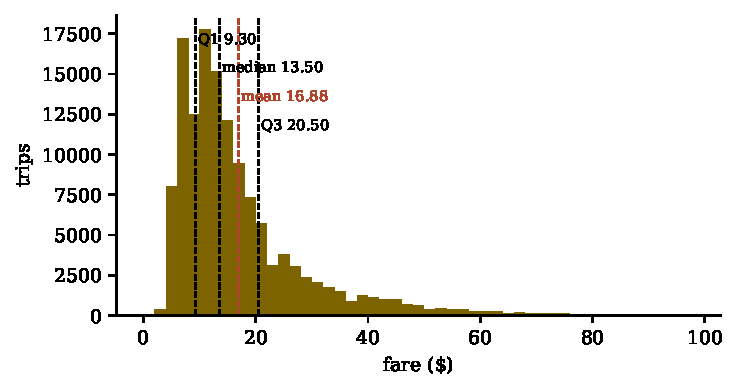
\includegraphics[width=\linewidth]{fare_hist}\caption{Fare distribution with quartiles and mean.}\end{subfigure}\hfill
\begin{subfigure}{0.49\linewidth}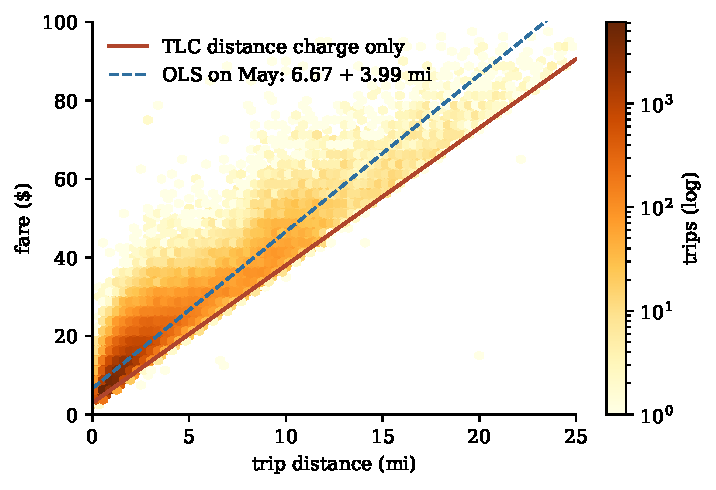
\includegraphics[width=\linewidth]{fare_vs_distance}\caption{Fare against distance (log density).}\end{subfigure}
\caption{May fares. The red line is the TLC distance charge alone; nearly all trips lie above it.}\label{fig:eda}
\end{figure}

\paragraph{Quartiles by trip type.} Distance is the first-order driver (Table~\ref{tab:quartiles}): the median fare rises from \usd{7.20} under one mile to \usd{84.20} above twenty. Time of day changes the price \emph{per mile} rather than per trip: the median fare per mile is about 40\% higher at midday than at night, while the median trip fare barely moves because night trips are longer. Airport trips are expensive (median \usd{44.30}) but cheap per mile (\usd{4.38}).
\TableQuartiles

\paragraph{The most expensive and the cheapest.} The highest median fares belong to airport pickups (LaGuardia, JFK and adjacent East Elmhurst), whose trips are long, followed by the southern tip of Manhattan, from which most destinations are far (Table~\ref{tab:rank-zone}). The cheapest pickup zones are the Upper East and Upper West Side, not because a mile is cheap there but because typical trips are short. Per mile, the most expensive trips are short hops within Times Square and Midtown at 4--5\,mph, up to \usd{15.74}/mi: the per-minute charge and the \usd{3} start dominate. The cheapest per mile are fast highway trips from JFK, close to the official \usd{3.50}/mi (Table~\ref{tab:rank-fpm}). Overall, \SlowShare\% of May trips average under 6\,mph, and their median fare per mile is \money{\SlowFpm} against \money{\MedianFpm} overall. For 1--5-mile trips the dearest mile is on weekdays between 11:00 and 17:00 and the cheapest at night (Figure~\ref{fig:time}).
\TableRankzone
\TableRankfpm

\begin{figure}[htbp]\centering
\begin{subfigure}{0.46\linewidth}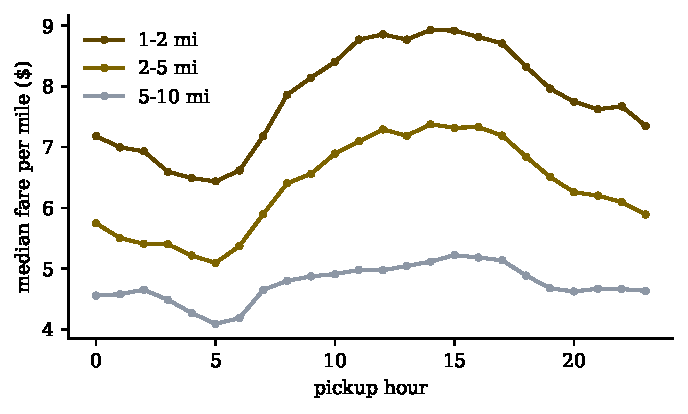
\includegraphics[width=\linewidth]{fpm_by_hour}\caption{Median \$/mi by hour and distance band.}\end{subfigure}\hfill
\begin{subfigure}{0.52\linewidth}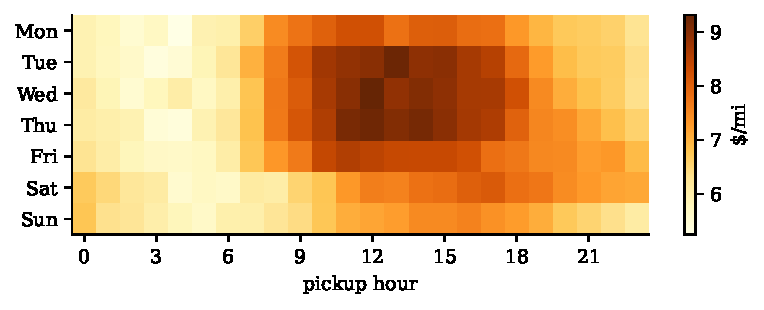
\includegraphics[width=\linewidth]{fpm_grid}\caption{Median \$/mi, 1--5 mi trips, weekday $\times$ hour.}\end{subfigure}
\caption{The time charge: the same mile costs more when traffic is slow (May).}\label{fig:time}
\end{figure}

\paragraph{Extremes removed by cleaning.} Before cleaning, 699 May trips (0.35\%) cost over \usd{100}. None survive: they are Nassau/Westchester, negotiated, flex, Newark and unknown-rate trips, plus 106 standard-meter trips beyond the 99.9\% caps (median 27\,mi). The ten most expensive cleaned trips sit just under the \usd{96.80} cap, and the ten cheapest pay the \usd{3.00} minimum after about one minute.

%=====================================================================
\section{Method}\label{sec:method}
\subsection{Leakage prevention}\label{sec:leak}
Two independent locks are enforced in \code{src/}.
\begin{enumerate}
  \item \textbf{Blacklist.} \code{FORBIDDEN} lists every post-trip field (drop-off time, duration, tip, total, tolls, all surcharges, rate code, payment type) and three fields excluded by decision (passenger count, vendor, request source). Any feature set naming one is rejected.
  \item \textbf{Whitelist enforced by construction.} The pipeline's first step selects only \code{BOOKING\_INPUTS} (pickup time, the two zone IDs, their boroughs, distance) before any feature is computed, so no feature can be derived from a post-trip column even by accident.
\end{enumerate}
A synthetic-data test suite (\code{python -m tests}, 15 tests) scrambles every forbidden column and checks that no prediction changes. It also checks that caps and encoders are fitted on the training month only, that seeded models are reproducible, and that the July lock admits exactly one scoring.

\subsection{Features}
Features are computed statelessly per trip; everything learned lives inside a scikit-learn \code{Pipeline} \cite{sklearn} and is therefore fitted on May only. Feature sets are cumulative (Table~\ref{tab:ablation}), so the ablation reads as ``what each addition did on June''. Zone identities are high-cardinality categoricals: 263 zones and several thousand observed pairs. They are encoded by smoothed target encoding \cite{micci} with 5-fold cross-fitting on the training data, so a training row never sees its own fare:
\begin{equation}
  \operatorname{TE}(c) = \lambda_c\,\bar y_c + (1-\lambda_c)\,\bar y, \qquad \lambda_c = \frac{n_c}{n_c + m},
\end{equation}
where $\bar y_c$ is the mean fare of category $c$ over the other folds, $\bar y$ the global mean, and $m$ the variance-based smoothing of \code{TargetEncoder}. Unseen categories receive $\bar y$. The final set \code{f7\_time\_x} also contains the distance split into ten time-of-week columns, $d\cdot\mathbb 1[\text{band}=b,\ \text{weekend}=w]$, which lets a linear model learn a per-mile price that varies with traffic.

\subsection{Models and baselines}
The baseline ladder consists of the May median fare, the official TLC rule ($3 + 3.5\,d$), a start-plus-per-mile line fitted on May, and a depth-2 tree. Candidate models are ordinary least squares, a CART regression tree, and histogram gradient boosting \cite{sklearn,lightgbm}. The final model minimises absolute error,
\begin{equation}
  \hat f = \arg\min_f \sum_{i\in\text{May}} \lvert y_i - f(x_i)\rvert ,
\end{equation}
so it estimates the conditional \emph{median} fare, which is the quantity MAE rewards. Final hyperparameters: loss \ParamLoss, learning rate \ParamLearningrate, \ParamMaxiter{} trees of at most \ParamMaxleafnodes{} leaves, at least \ParamMinsamplesleaf{} trips per leaf, seed 0.

\subsection{Evaluation protocol}\label{sec:protocol}
\begin{enumerate}
  \item \textbf{Metrics.} The primary metric is MAE in dollars; RMSE (sensitive to the tail) and bias $\overline{y-\hat y}$ are secondary.
  \item \textbf{Selection rules, fixed before the comparisons ran.} Hyperparameters: the cheapest setting (fewest leaves, then fewest iterations) within \usd{0.01} of the best June MAE. Model: the lowest June MAE, unless its gain over the next simpler candidate has a 95\% interval that includes 0.
  \item \textbf{Uncertainty.} Trips on the same day share weather, traffic and events, so resampling single trips would understate uncertainty. We use a day-block percentile bootstrap \cite{efron,kunsch}: with day blocks $b=1..B$ and per-block sums $S_b$ of absolute and squared errors, each replicate draws $(w_1,\dots,w_B)\sim\text{Multinomial}(B,\tfrac1B)$ and recomputes MAE and RMSE from $\sum_b w_b S_b$, for the model and the comparator jointly (paired). 2\,000 replicates; 95\% percentile intervals; $B=30$ (June) or 31 (July).
  \item \textbf{July is scored once.} A lock file written by \code{lock\_test()} makes a second scoring raise an error.
\end{enumerate}

\subsection{From prediction to quote}
A quote rule maps a prediction $\hat y$ to a price $q$ with target coverage $P(y\le q)=0.9$. Three rules were compared: an additive buffer $q=\hat y+b$, a multiplicative one $q=\max(\hat y,3)\,k$, and a per-distance-band buffer $q=\hat y+b_{\text{band}}$, with $b$ the 90th percentile of June residuals in the band. A rule fitted and scored on the same trips hits 90\% by construction, so the rules were compared by \emph{cross-fitting} within June: fit on odd days, score on even days, and vice versa. The criterion, fixed in advance, was the smallest worst-slice coverage gap $\max_s\lvert\text{cov}_s-0.9\rvert$ over distance band, time of day, airport flag and pickup borough (slices with $n\ge1000$), with ties broken by the lower mean cushion.

%=====================================================================
\section{Results}\label{sec:results}
\subsection{Feature ablation and tuning (June)}
\TableAblation
Hour and weekday help every model, most of all the boosted model (\usd{2.800}$\to$\usd{2.499}). Boroughs and airport flags add little because 93\% of pickups are in Manhattan. The decisive addition is the zone target encoding (HGB \usd{2.434}$\to$\usd{2.259}), followed by the zone pair and the time$\times$distance terms (Table~\ref{tab:ablation}, Figure~\ref{fig:ablation}). No feature group made any model worse.

The tree's optimum in the original skeleton grid lay on the grid edge; the extended grid shows a plateau (depth 14--20 within \usd{0.02}). For gradient boosting, absolute-error loss beats squared error throughout (best \usd{2.077} vs \usd{2.145}). The top ten of 64 settings span less than one cent (Appendix, Table~\ref{tab:hgbgrid}), and the parsimony rule selects the setting reported above, at a June cost of \usd{0.009}.

\begin{figure}[htbp]\centering
\begin{subfigure}{0.49\linewidth}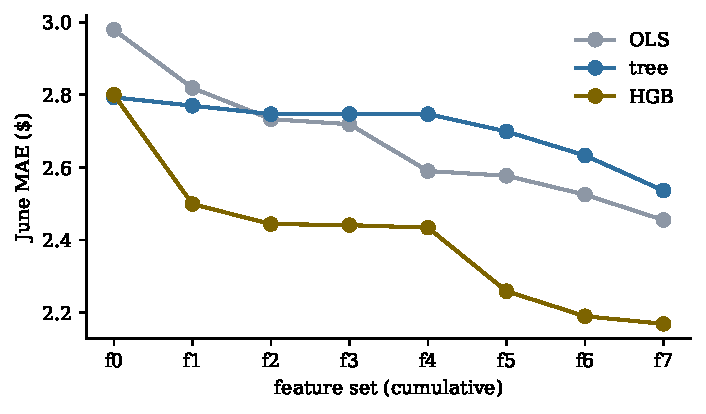
\includegraphics[width=\linewidth]{ablation}\caption{June MAE by cumulative feature set.}\label{fig:ablation}\end{subfigure}\hfill
\begin{subfigure}{0.49\linewidth}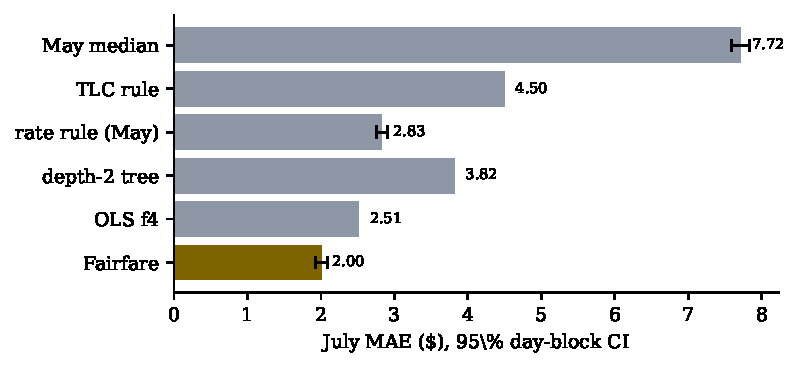
\includegraphics[width=\linewidth]{july_mae}\caption{July MAE with 95\% day-block intervals.}\label{fig:julymae}\end{subfigure}
\caption{Model development on June and the final comparison on July.}
\end{figure}

\subsection{Model selection (June)}
\TableSelection
The paired June MAE difference between the boosted model and the best simpler candidate, the depth-20 tree, is \money{\SelTreeMaePoint} per trip (95\% CI \money{\SelTreeMaeLo} to \money{\SelTreeMaeHi}); against the linear model it is \money{\SelLinearMaePoint} and against the fitted rate rule \money{\SelRuleMaePoint}. All intervals exclude zero, so the rule retains gradient boosting. Because June served for feature choice, tuning and this comparison, the winner's June error (\money{\JuneFinalMae}) is optimistic. July is the unbiased estimate.

\subsection{Final evaluation (July)}
\TableLadder
On \JulyN{} July trips, scored once on \JulyScoredAt, the final model reaches MAE \money{\JulyFinalMae} (95\% CI \money{\JulyVsMedianMaemodelLo}--\money{\JulyVsMedianMaemodelHi}), RMSE \money{\JulyFinalRmse} (\money{\JulyVsMedianRmsemodelLo}--\money{\JulyVsMedianRmsemodelHi}) and bias \money{\JulyFinalBias} (Table~\ref{tab:ladder}, Figure~\ref{fig:julymae}). The paired difference to the fitted rate rule is \money{\JulyVsRuleMaediffPoint} per trip in MAE (CI \money{\JulyVsRuleMaediffLo} to \money{\JulyVsRuleMaediffHi}) and \money{\JulyVsRuleRmsediffPoint} in RMSE (\money{\JulyVsRuleRmsediffLo} to \money{\JulyVsRuleRmsediffHi}); to the median baseline it is \money{\JulyVsMedianMaediffPoint} in MAE (\money{\JulyVsMedianMaediffLo} to \money{\JulyVsMedianMaediffHi}). The official distance-only rule under-predicts by \money{\JulyTlcBias} on average: almost five dollars of time charge per trip.

\paragraph{Error structure.} Residuals are centred near zero with a long right tail (Figure~\ref{fig:resid}). Calibration by prediction decile stays close to the diagonal: the cheapest decile is slightly under-predicted and the most expensive slightly over-predicted. Grouping July trips by their realised average speed, an analysis-only quantity, isolates the source of the error. Trips slower than 6\,mph are under-predicted by \usd{2.52} on average, while fast trips are over-predicted (Table~\ref{tab:slices}). The per-minute charge is the part of the fare that booking-time inputs cannot see.

\begin{figure}[htbp]\centering
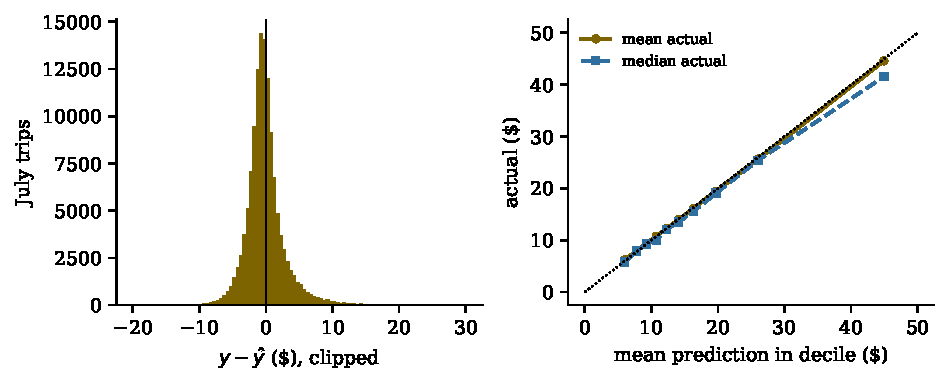
\includegraphics[width=0.92\linewidth]{july_residuals}
\caption{July: residual distribution (left) and calibration by prediction decile (right).}\label{fig:resid}
\end{figure}

\subsection{The quote}
\TableRules
The per-band rule gave the most even coverage under cross-fitting and the smallest cushion (Table~\ref{tab:rules}). Its frozen buffers grow with distance (Table~\ref{tab:buffers}). On July it covers \JulyQuoteCoverage{} of trips (June: \JuneQuoteCoverage{}), with an average cushion (quote minus fare) of \money{\JulyQuoteMeancushion}. When the fare exceeds the quote, it does so by \money{\JulyQuoteMeanshortfallwhenunder} on average. Every slice with at least 500 trips reaches at least 90.4\% coverage (Table~\ref{tab:slices}). The exception is trips over 20 miles (201 trips, 72.1\%), whose band had fewer than 200 June trips and fell back to the smaller global buffer. This known weakness was reported, not fixed after July. Coverage is highest at night and tightest on weekday afternoons (Figure~\ref{fig:hour}).
\TableBuffers
\TableSlices

\begin{figure}[htbp]\centering
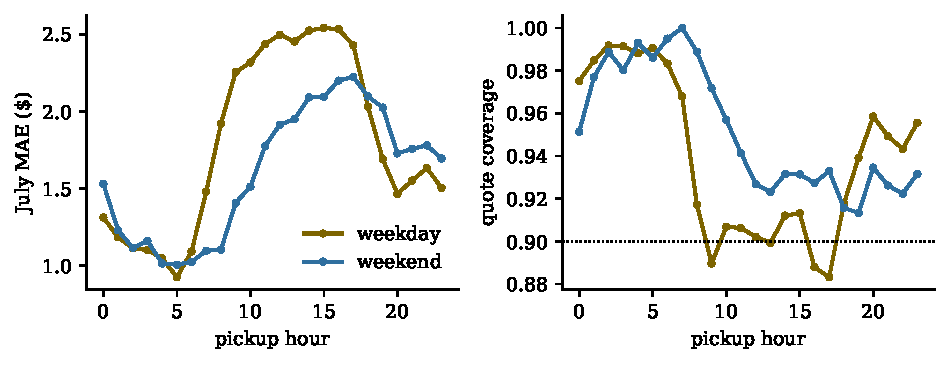
\includegraphics[width=0.92\linewidth]{july_hour}
\caption{July MAE and quote coverage by pickup hour, weekday vs weekend.}\label{fig:hour}
\end{figure}

\begin{figure}[htbp]\centering
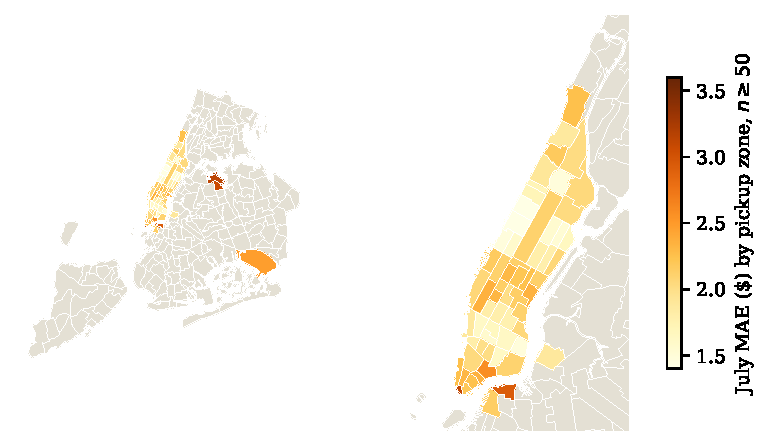
\includegraphics[width=0.95\linewidth]{zone_map}
\caption{July MAE by pickup zone (zones with $n\ge50$; grey: fewer trips). Left: all of NYC; right: Manhattan.}\label{fig:map}
\end{figure}

\subsection{Distribution shift}
July fares ran slightly below what the May-trained model expects: the bias moved from $+$\money{\JuneFinalBias} (June) to \money{\JulyFinalBias} (July), and the fitted rate rule drifted in the same direction (\money{\JuneRuleBias}$\to$\money{\JulyRuleBias}). As a result the June-calibrated quote over-covers in July. Plausible causes, which this design cannot test, are lighter summer traffic and school holidays. The population itself also drifts (growing flex share, vendor-specific rate-code artefacts) without changing the definition of a metered trip.

%=====================================================================
\section{The planned-distance assumption and a booking-time routing estimate}\label{sec:routing}
\paragraph{Sensitivity.} The data's \code{trip\_distance} is an odometer reading taken after the trip, whereas an app only has a routed estimate. Feeding the June trips distances perturbed by mean-one log-normal noise shows how much this matters (Table~\ref{tab:noise}): a 10\% routing error raises the MAE by about 22 cents and lowers coverage to 89.3\%.
\TableNoise

\paragraph{A straight-line router.} To make the predictor usable without a routing service, the website estimates the planned distance from the zone centroids $c_i$ (area-weighted, computed from the TLC shapefile in NY State Plane feet):
\begin{equation}
 \hat d_{ij} = k_{\beta(s_{ij})}\, s_{ij},\qquad s_{ij} = \lVert c_i - c_j\rVert_2, \qquad
 k_\beta = \operatorname{median}\left\{\frac{d_t}{s_t} : t\in\text{May},\ i_t\ne j_t,\ \beta(s_t)=\beta\right\},
\end{equation}
where $\beta(\cdot)$ is the straight-line length band. Same-zone trips use the zone's median May distance. A single factor ($k=\RouterK$) under-estimated long trips, so the factor depends on length: it is 1.79 for very short hops, 1.17--1.28 for 1--5\,mi, and 1.35--1.46 beyond, where bridges and highways add detour. On June the estimate is off by \RouterDistMae{}\,mi on average (median error \RouterDistMape\%; Figure~\ref{fig:router}).

\paragraph{What it costs.} Fed the estimate, the frozen model's June MAE rises from \money{\RouterOdoMae} to \money{\RouterEstMae}, and the original buffers would cover only \RouterEstCov\% (Table~\ref{tab:router}). Estimated distances therefore receive their own per-band buffers, fitted the same way on June (Table~\ref{tab:buffers}), which restore \RouterXfitCov\% cross-fitted coverage at an average cushion of \money{\RouterXfitCushion}. Two alternatives were measured but not adopted: retraining on estimated distances (\money{\RouterRetrainedMae}) and using the May median distance of the zone pair (\money{\RouterPairMae}). This mode was added after the final July run and has been evaluated on June only.
\TableRouter

\begin{figure}[htbp]\centering
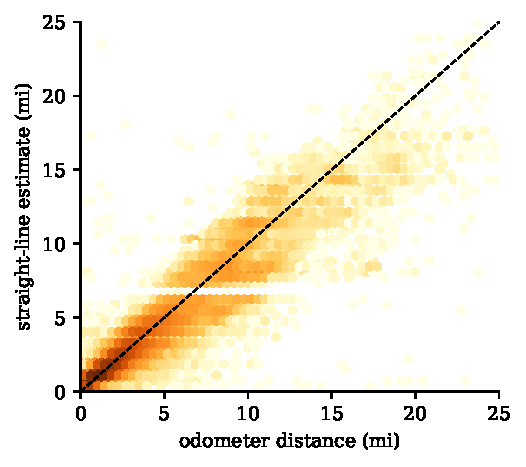
\includegraphics[width=0.42\linewidth]{router}
\caption{June: straight-line estimate against odometer distance.}\label{fig:router}
\end{figure}

%=====================================================================
\section{Software and the interactive website}
The pipeline lives in a Python package (\code{src/}) whose functions are imported by five stage notebooks (frame, clean and split, features, evaluate, routing and EDA). Small result files are committed under \code{results/}, and every number in this report and on the website is generated from them by scripts. The website (\code{site/}, Vite + React + TypeScript, static) contains a fare predictor that evaluates the frozen model \emph{in the browser}. An export script writes the fitted one-hot categories, target-encoding tables and all trees to JSON, and a TypeScript port reproduces the feature code and tree traversal. On 2\,000 June trips the browser and scikit-learn predictions agree exactly (maximum difference 0), and the routing estimate agrees to $10^{-14}$\,mi. The site is deployed to GitHub Pages only by a manually triggered workflow.

%=====================================================================
\section{Discussion and limitations}
\begin{itemize}
  \item \textbf{Optimistic distance.} Training and testing on odometer distance makes the headline numbers optimistic. Section~\ref{sec:routing} brackets the cost between a perfect router and a straight-line estimate.
  \item \textbf{Scope defined after the fact.} The population uses post-trip fields, which a deployment must replace by knowing that the trip is metered.
  \item \textbf{Unobservable time.} The per-minute charge is the dominant residual error. Real-time traffic speeds by zone and hour are the most promising additional input.
  \item \textbf{Quote design.} A buffer per distance band leaves coverage uneven by time of day (97.8\% at night vs 91.3\% midday). Quantile regression for the 90th percentile, or buffers by band $\times$ time, would even it out, and the 20+\,mi band needs a non-global fallback.
  \item \textbf{Evaluation history.} An early skeleton notebook scored July once on 2026-11-01, before any model or buffer was frozen (OLS, MAE \usd{2.512}). All later choices were made on June. With the project owner's approval the lock was reset, and the frozen configuration was scored once on \JulyScoredAt. Both runs are recorded in the repository history; we report this as a protocol deviation.
  \item \textbf{External validity.} Three months of one year, one city, one sample. Seasonality and fare-rule changes beyond July 2026 are untested.
\end{itemize}

%=====================================================================
\section{Conclusion}
Booking-time inputs predict the NYC yellow-taxi meter fare to within about two dollars on a month the model never saw, with a 30\% lower error than the best simple rule, and a per-distance-band buffer turns the prediction into a quote that held for \JulyQuoteCoverage{} of July trips. What remains is mostly the price of time in traffic. The methodological contribution matters as much as the model: an explicit population, leakage guards enforced by construction and tested, pre-stated selection rules, honest intervals, and a test month that could only be looked at once.

%=====================================================================
\section*{Reproducibility}
\begin{verbatim}
pip install -r requirements.txt   # pinned versions (Python 3.12)
python data/get_data.py           # download + SHA-256 verification
python -m tests                   # 15 protocol tests on synthetic data
cd notebooks && jupyter nbconvert --to notebook --execute --inplace 0*.ipynb
python documentation/make_report_assets.py      # figures, numbers, tables
cd documentation && tectonic fairfare_report.tex   # PDF
\end{verbatim}
All random procedures are seeded (seed 0). NB04 refuses to score July a second time in this repository; in a fresh clone it reproduces the reported numbers.

%=====================================================================
\section*{Author contributions}
\begin{tabular}{@{}p{0.24\linewidth}p{0.72\linewidth}@{}}
\toprule
\textbf{Blevis Allushi} & \textbf{Project lead, protocol and pipeline.} Set up the repository, the \code{src/} package and the five-stage pipeline; designed the evaluation protocol (temporal split, pre-stated selection rules, single-use July lock); data acquisition, cleaning and the population definition; hyperparameter tuning and the single July run; the booking-time distance (routing) study; directed the website; wrote the report. \\
\midrule
\textbf{Geri Belba} & \textbf{Features and leakage.} Ran the May exploratory analysis (fare per mile by hour, weekday, borough and zone; airport trips) that motivated the time and zone features; designed the cumulative feature ladder and its June ablation, including the target-encoded zone pair and the distance $\times$ time-of-week interactions; audited every feature against the leakage blacklist; reviewed the distance-noise sensitivity analysis. \\
\midrule
\textbf{Leandra Latifi} & \textbf{Evaluation and the quote.} Built the baseline ladder (median, fitted rate rule, shallow tree) and the slice analysis; designed the comparison of quote rules (additive, multiplicative, per distance band) with odd/even-day cross-fitting on June; analysed July coverage and the failure modes (slow traffic, 20+\,mi trips, airports); wrote the model card. \\
\bottomrule
\end{tabular}

\section*{Use of generative AI}
Generative AI (Anthropic's Claude, used through the Claude Code assistant) was used in this project as follows. The \textbf{project website} (\code{site/}) was generated with AI from our specifications, including the in-browser model port and its parity test. For the \textbf{analysis code}, AI worked from the pipeline the team had already written (data loading, cleaning, the first feature sets, the baselines and the evaluation helpers) and helped extend it: additional feature sets and model options, the quote-rule and distance-perturbation helpers, the protocol tests and the straight-line distance estimator. It also helped edit the notebook narratives and the Markdown documentation. Every methodological decision (population scope, temporal protocol, selection rules, the reset of the July lock) was made or explicitly approved by the team; Blevis Allushi reviewed all AI-produced code, ran every analysis and checked the reported numbers against the executed outputs. All results come from code executed in the repository; none were produced or altered by hand. AI is not an author of this work.

%=====================================================================
\begin{thebibliography}{9}\small
\bibitem{tlcfare} NYC Taxi \& Limousine Commission. \emph{Taxi fare} (Rate \#01 standard city rate). \url{https://www.nyc.gov/site/tlc/passengers/taxi-fare.page}, accessed 15 November 2026.
\bibitem{tlcdict} NYC Taxi \& Limousine Commission. \emph{Data dictionary -- yellow taxi trip records}. Distributed with the course data release.
\bibitem{sklearn} F.~Pedregosa et al. Scikit-learn: Machine learning in Python. \emph{Journal of Machine Learning Research}, 12:2825--2830, 2011.
\bibitem{lightgbm} G.~Ke et al. LightGBM: A highly efficient gradient boosting decision tree. In \emph{Advances in Neural Information Processing Systems 30}, 2017.
\bibitem{micci} D.~Micci-Barreca. A preprocessing scheme for high-cardinality categorical attributes in classification and prediction problems. \emph{ACM SIGKDD Explorations}, 3(1):27--32, 2001.
\bibitem{efron} B.~Efron and R.~J.~Tibshirani. \emph{An Introduction to the Bootstrap}. Chapman \& Hall, 1993.
\bibitem{kunsch} H.~R.~K\"unsch. The jackknife and the bootstrap for general stationary observations. \emph{The Annals of Statistics}, 17(3):1217--1241, 1989.
\end{thebibliography}

\appendix
\section{Hyperparameter search}
\TableHgbgrid
\end{document}
